\documentclass[conference]{IEEEtran}
\usepackage{graphicx}
\usepackage{amsmath}
\usepackage{caption}
\usepackage{float}

% Title and author
\title{Performance of SPMV Calculation using OpenMPI}
\author{Charlie Flux}

\begin{document}
\maketitle

\begin{abstract}
This paper investigates the performance of sparse matrix-vector multiplication (SPMV) using naive and structured approaches using OpenMPI. This paper focuses on the COO-to-CSR conversion and workload partitioning. 
\end{abstract}

\section{Introduction}
The purpose of this experiment is to compare the performance of naive and structured implementations of SPMV using OpenMPI. Specifically, it examines how varying rank counts affect the performance of distributed sparse matrix-vector multiplication algorithms.
\section{Methodology}
2 Approaches of calculating SPMV were used:
\begin{itemize}
    \item \textbf{Naive}
    \item \textbf{Strucuted COO-to-CSR conversion with reduction} 
\end{itemize}

For experiments, measuring time, rank counts \(R\) were chosen from the set:
    \[
    R = \{1, 2, 4, 6, 8, 12, 16, 24, 32\}
    \]
All experiments used the arguments the matricies provided by cant.mtx \& b.mtx files.
\subsection{Experimental Setup}
All tests were ran on Talepas. Experiments were repeated 10 times and the average was calculated for each experiment. \\
Data was filtered using the Interquartile Range Filter to remove points that do not lie between the first and third quartile as a consequence of the the unreliable data caused by the unlocked variable frequencies on Telepas.

\section{Results}

\subsection{Broadcast}
The first stage of both methods is to broadcast data out to all nodes. Both the naive and structured approach perform similarly. This is expected as the data that is broadcasted is the same therefore, with no differences in implementation, similar results are expected.
\begin{figure}[H]
    \centering
    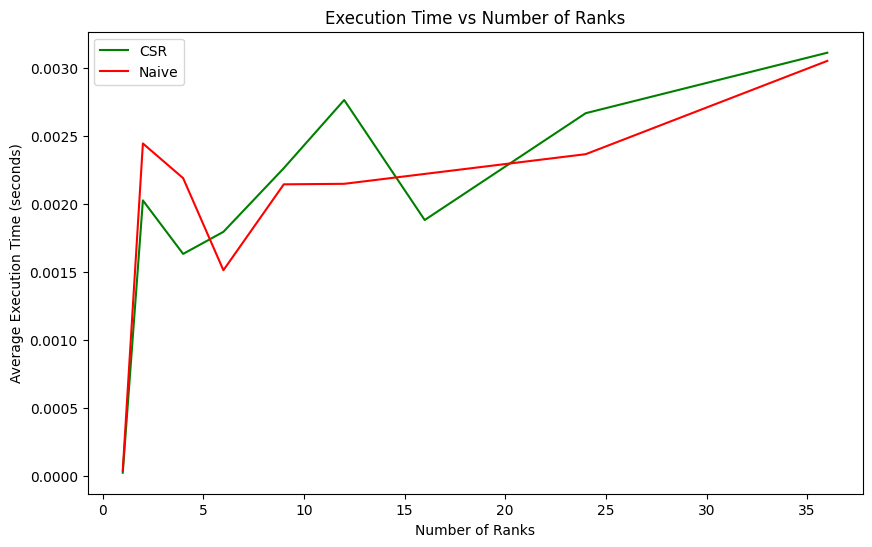
\includegraphics[width=0.45\textwidth]{../img/broadcast.png}
    \caption{SPMV GPU Implementations}
    \label{fig:zoomed}
\end{figure}

\subsection{Scatter}
The next stage is to scatter the rows that each node will be processing out. The CSR format performs better than the COO format during the scatter due to the reduced amount data that is needed to store the matrix. I implemented load balancing on the rows by calculating an equal amount of non zero values for each node to process, this should result in a speedup during the SPMV calculation.
\begin{figure}[H]
    \centering
    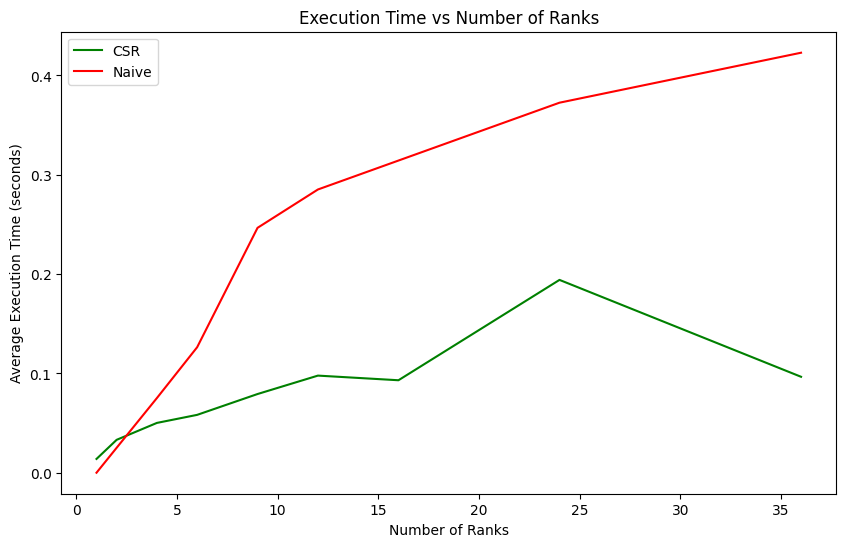
\includegraphics[width=0.45\textwidth]{../img/scatter.png}
    \caption{CSR implementation}
    \label{fig:parallel}
\end{figure}

\subsection{SPMV}
The SPMV section of the code is similar in distribution however, the structured approach uses load balancing which is apparent in Figure \ref{fig:spmv}. The structured approach sees an improvements as the number of ranks increases whereas, the naive approach suffers as more nodes are introduced. I believe that the naive approach suffered because of the lack of load balancing therefore, some nodes will have a more work to do than other which increases the wait time on a single node.
\begin{figure}[H]
    \centering
    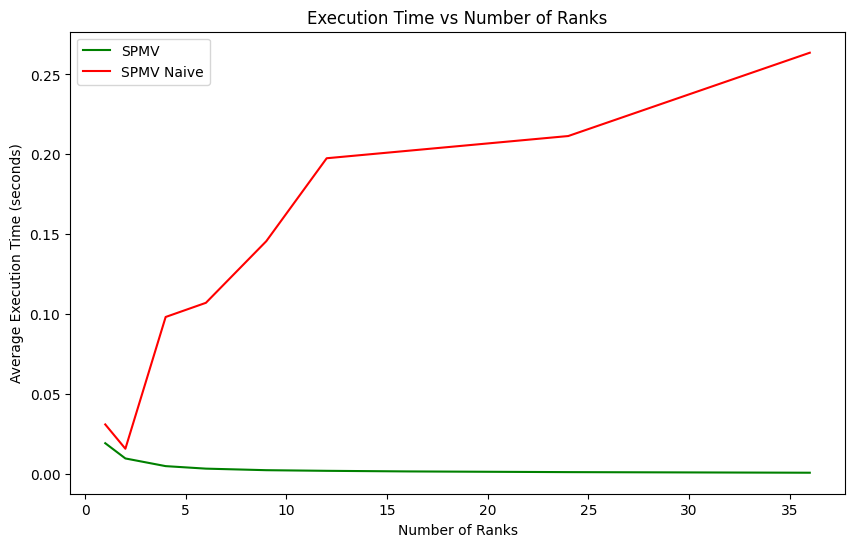
\includegraphics[width=0.45\textwidth]{../img/spmv.png}
    \caption{SPMV Calculation}
    \label{fig:spmv}
\end{figure}

\subsection{Reduction}
The final stage of the SPMV calculation is the reduction on rank 0. The structured approach performs better than the naive approach as the number of nodes increases. I did not implement reduced local result array sizes which would offer a greater speedup on the structured compared to naive approach.
\begin{figure}[H]
    \centering
    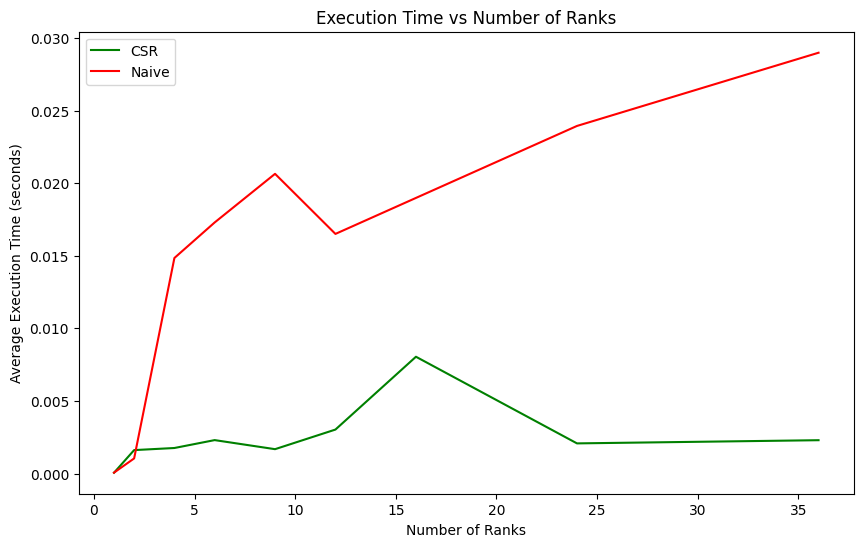
\includegraphics[width=0.45\textwidth]{../img/reduce.png}
    \caption{COO to CSR Conversion}
    \label{fig:conversion}
\end{figure}

\section{Conclusion}
This experiment compared the performance of SPMV matrix calucations using OpenMPI focusing on a structured vs naive approach. 
In conculsion the structured approach performed better across the board.
This performance difference is due to the reduced data used by the CSR matrix format, effective load balancing which minimizes idle time and ensures more efficient workload distribution.
However, further optimization, such as reducing local result array sizes, could enhance performance.
\end{document}
